\documentclass[12pt]{beamer}
\usepackage[T1, T2A]{fontenc}
\usepackage[utf8]{inputenc}
\usepackage[english,russian]{babel}
\usepackage{amssymb,amsfonts,amsmath,mathtext}
\usepackage{cite,enumerate,float,indentfirst}
\usepackage{listings}

\graphicspath{{images/}}

\usetheme{Pittsburgh}
\usecolortheme{whale}

\setbeamercolor{footline}{fg=blue}
\setbeamertemplate{footline}{
  \leavevmode%
  \hbox{%
  \begin{beamercolorbox}[wd=.333333\paperwidth,ht=2.25ex,dp=1ex,center]{}%
    Занятие 1
  \end{beamercolorbox}%
  \begin{beamercolorbox}[wd=.333333\paperwidth,ht=2.25ex,dp=1ex,center]{}%
    8 февраля 2018
  \end{beamercolorbox}%
  \begin{beamercolorbox}[wd=.333333\paperwidth,ht=2.25ex,dp=1ex,right]{}%
  Стр. \insertframenumber{} из \inserttotalframenumber \hspace*{2ex}
  \end{beamercolorbox}}%
  \vskip0pt%
}

\graphicspath{{../../images/}}

\newcommand{\itemi}{\item[\checkmark]}

\title{\small{Интеллектуальные системы управления в робототехнике}}
\author{\small{%
\emph{Занятие 1} \\Архитектура системы управления робототехнической системой\\}%
\vspace{30pt}%
МФТИ\\
ФИЦ ИУ РАН%
\vspace{20pt}%
}
\date{\small{8 февраля, 2018}}

\begin{document}

\maketitle

\begin{frame}
\frametitle{План на сегодня}
\tableofcontents 
\end{frame}


\section{Формальные требования}

\begin{frame}
\frametitle{План на сегодня}
\tableofcontents[currentsection] 
\end{frame}

\begin{frame}
\frametitle{Цель курса}
	\begin{enumerate}
		\item Понять, что такое роботы и как с ними работать.
		\item Разобраться с тем, какие методы существуют, чтобы сделать роботов более автономными.
		\item Попрактиковаться в работе с этими методами с реальными примерами.
		\item Выполнить исследовательский проект.
		\item Познакомиться с основными научными проблемами в этой области и подходами к их решению. 
	\end{enumerate}
	\centering
	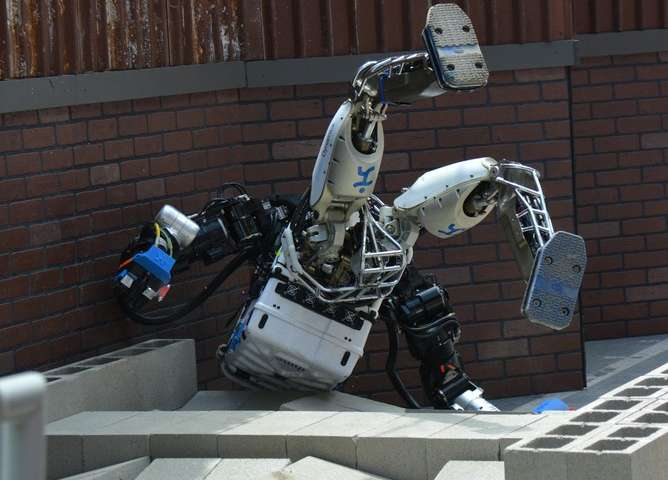
\includegraphics[width=0.4\linewidth]{robot_crash.jpg}
\end{frame}

\begin{frame}
\frametitle{Разделы курса}
\begin{enumerate}
	\item Интеллектуальное управление (устойчивость, управляемость, стабилизируемость,детектирвоание, помехи, фильтры).
	\item Планирование траекторий (A*, статическая среда, ограничения по модели, многоагентный подход).
	\item Когнитивные функции (память, обучение, методы аппроксимации, планирование поведения).
\end{enumerate}
	\centering
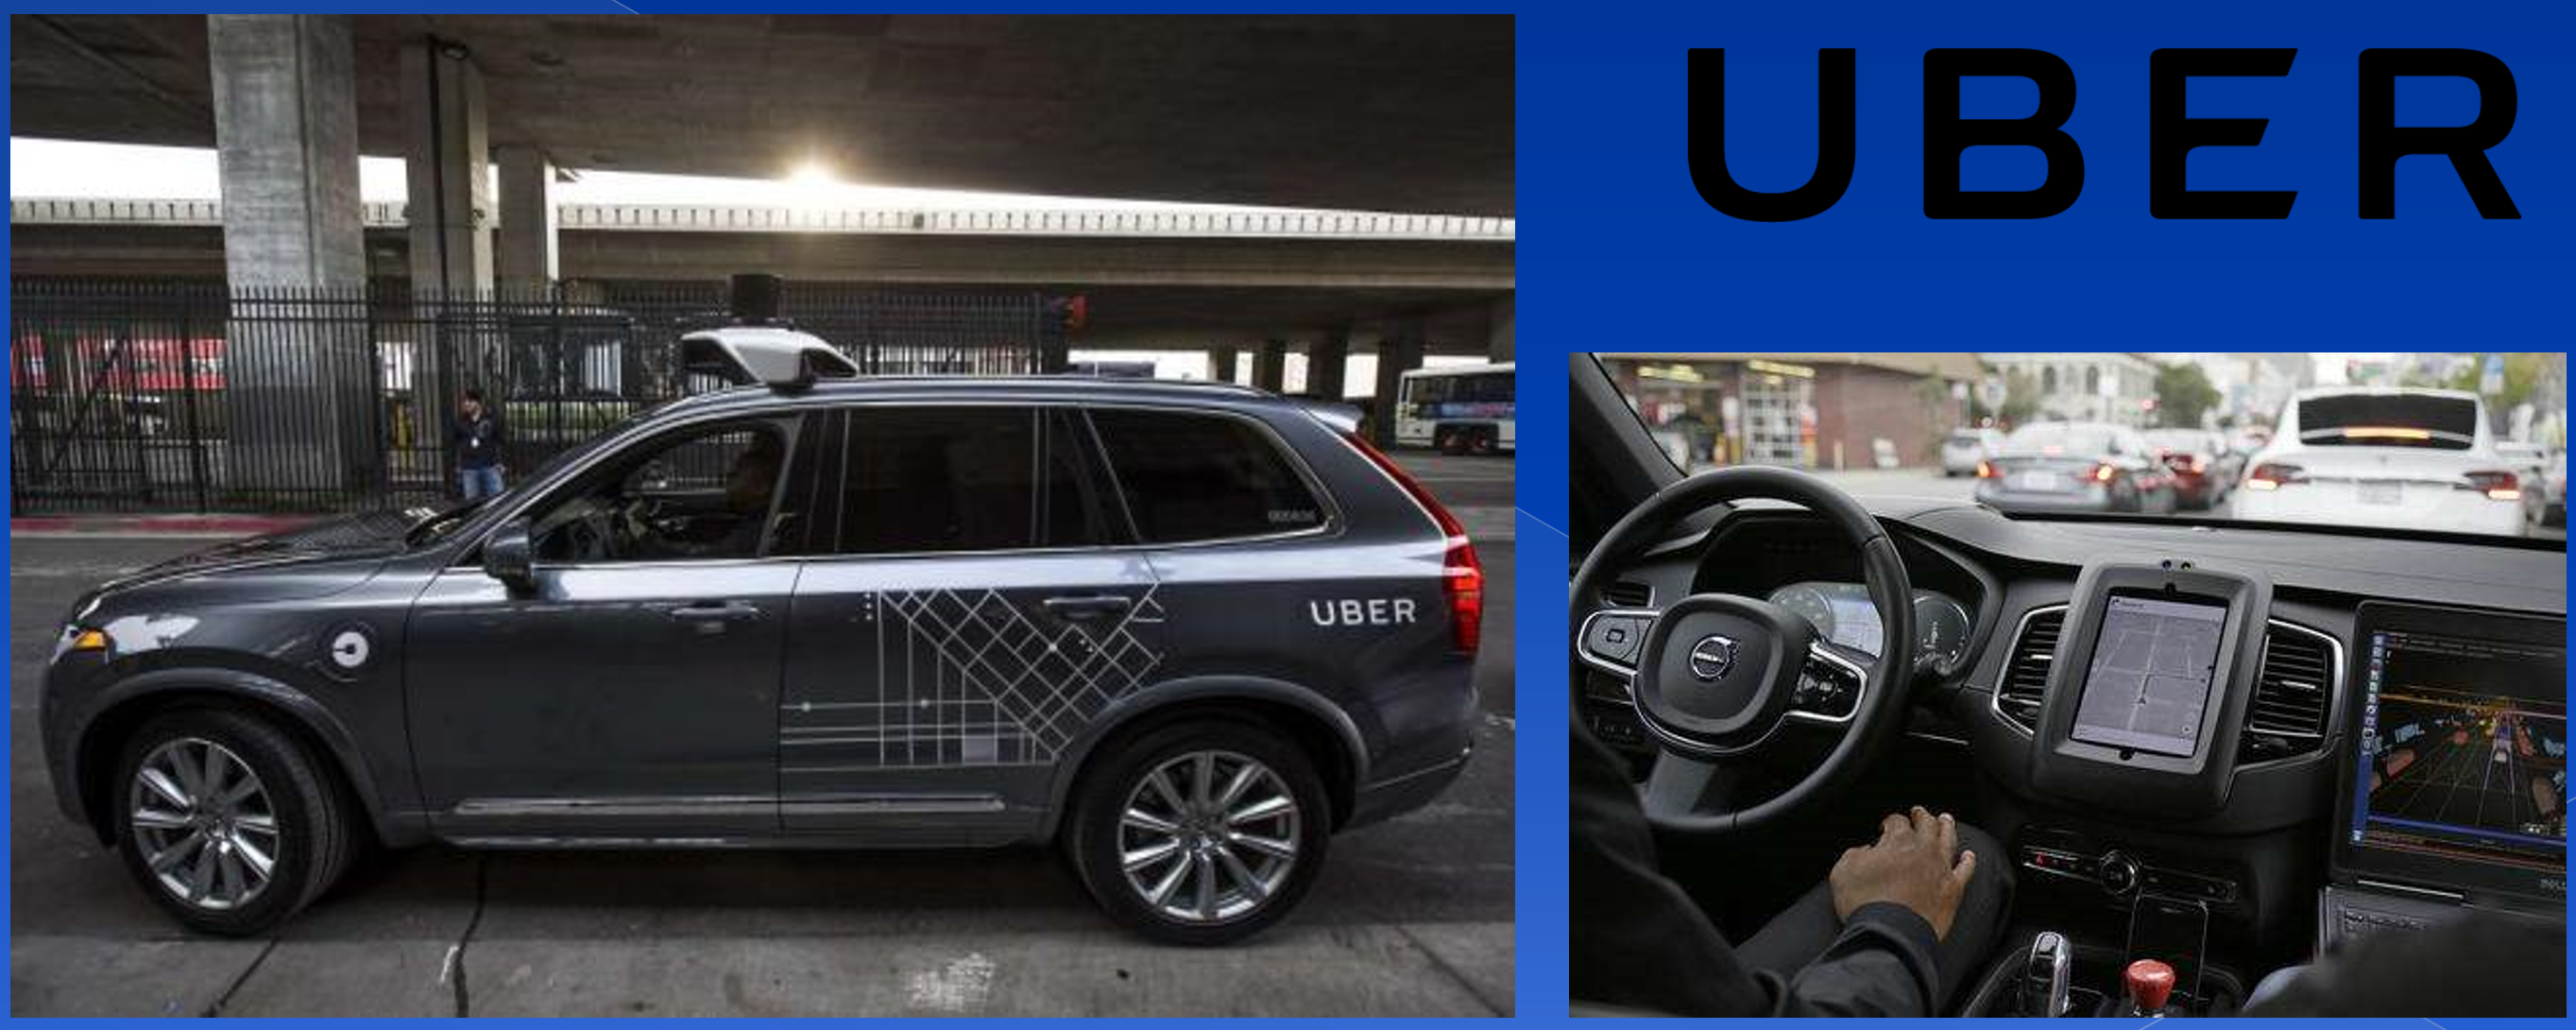
\includegraphics[width=0.75\linewidth]{uber.png}
\end{frame}

\begin{frame}
\frametitle{Формальные требования}
\begin{itemize}
	\item Формула оценки: \[O_{\text{итог}}=0.6\sum_{N=1}^3 O_{\text{ДЗ}_N}+0.4\cdot O_{\text{проект}}\]
	\item По каждому разделу курса буду лабораторные работы, на которых будут разбираться задачи, похожие на ДЗ - \textbf{нужны ноутбуки!}
	\item Можно выбрать одну тему проекта, выполнить его и оформить результаты в виде отчета и защитить его в конце семестра.
	\item Все материалы по курсу будут выкладывать на странице \href{https://piazza.com/class/jdd7dvwvvwv7kq}{Piazza}, тем же можно задавать вопросы.
\end{itemize}

\end{frame}

\begin{frame}
\frametitle{О лаборатории 0-2: состав}
	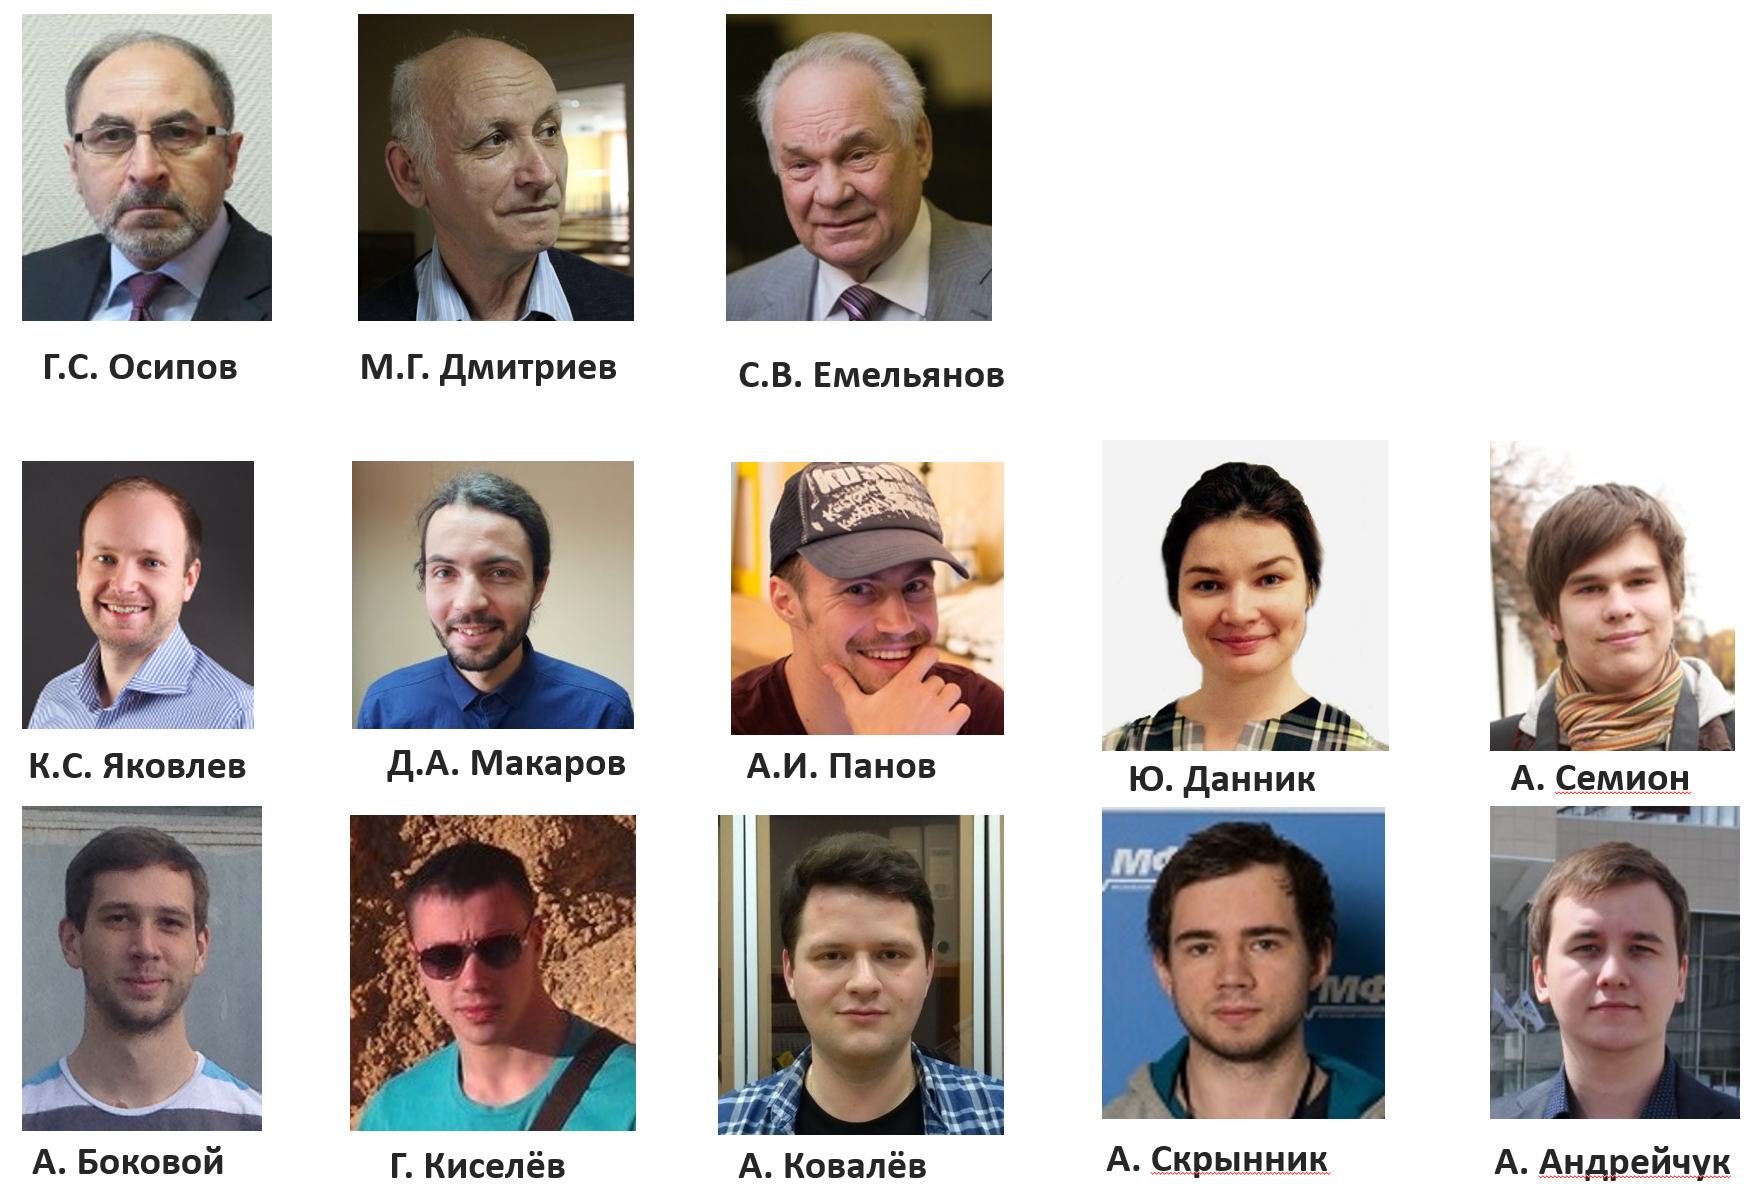
\includegraphics[width=1\linewidth]{lab02.png}
\end{frame}

\begin{frame}
\frametitle{О лаборатории 0-2: темы и проекты}
	\scriptsize
	\begin{columns}
		\begin{column}{0.7\textwidth}
			\begin{itemize}
				\item Управление нелинейными системами с помощью численно-аналитических методов
				\item Сингулярно возмущенные системы управления
				\item Экономичные разностные схемы
				\item Поиск пути с учетом геометрических ограничений
				\item Планирование альтернативных траекторий
				\item Картирование и локализация по видеопотоку единственной камеры
				\item Моделирование когнитивных функций (планирование, целеполагание, рефлексия, мотивация)
				\item Методы машинного обучения (обучение с подкреплением - иерархическое, глубокое, мультиагентное)
				\item Нейросимвольные архитектуры
				\item Представление пространственных и временных знаний
				\item Планирование коалиционного и коллаборативного поведения (распределение ролей и ассистенты)
				\item Моделирование рассуждений в картине мира 
			\end{itemize}
		\end{column}
		\begin{column}{0.3\textwidth}
			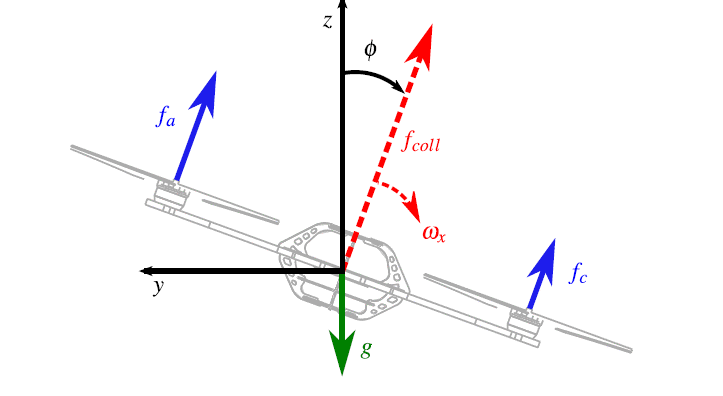
\includegraphics[width=\textwidth]{proj1.png}
			
			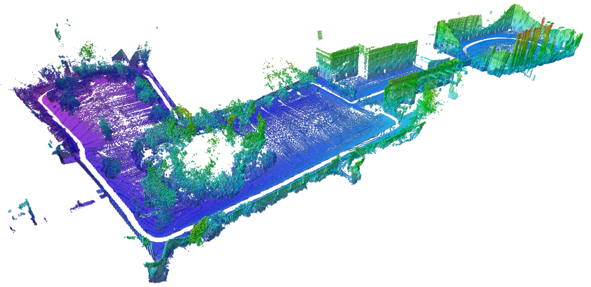
\includegraphics[width=\textwidth]{proj2.png}
			
			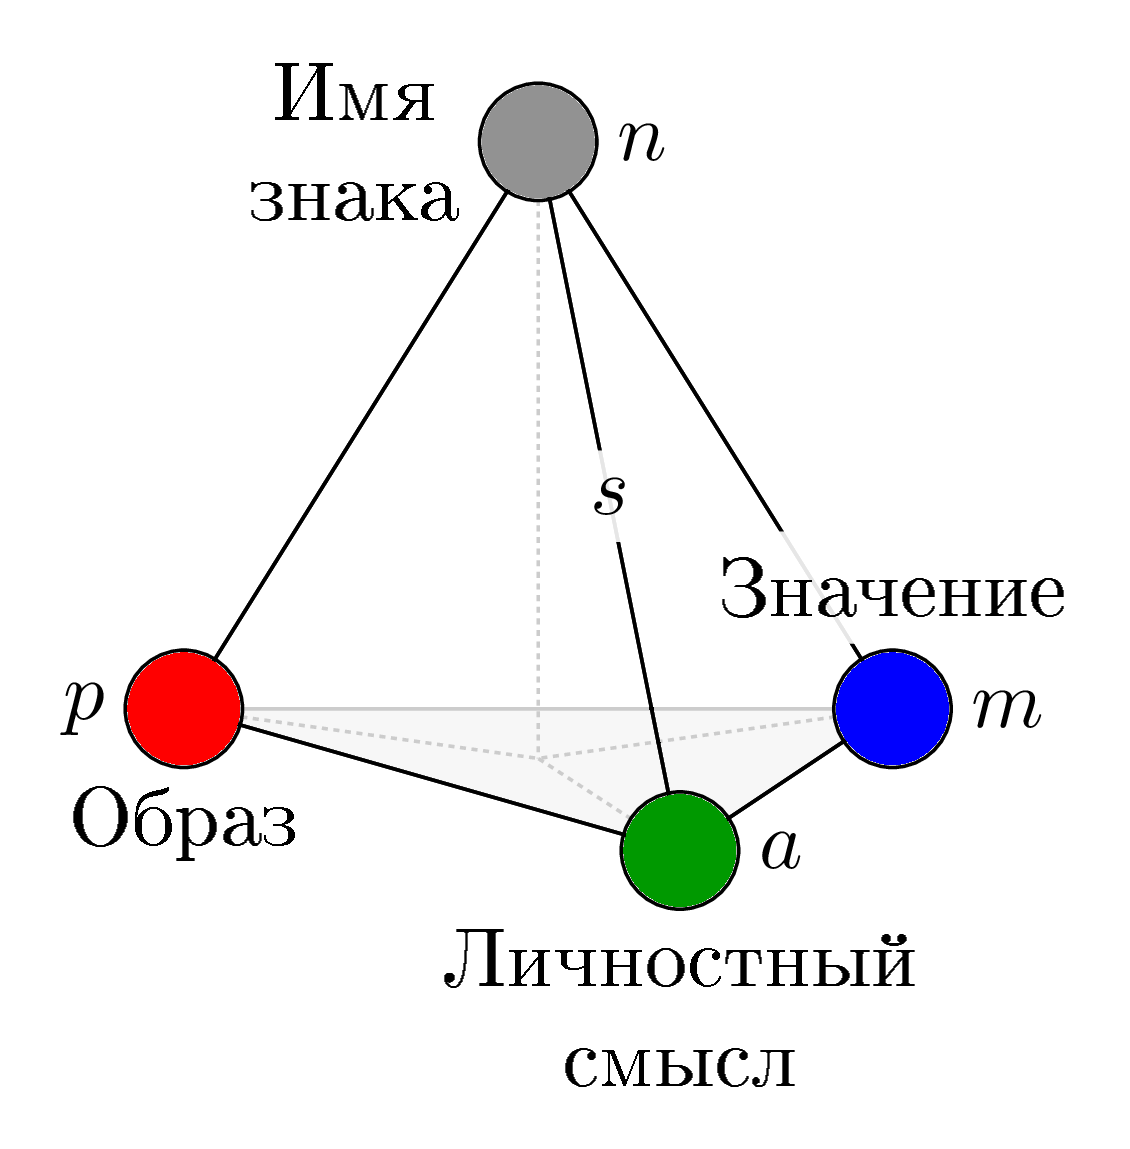
\includegraphics[width=0.8\textwidth]{sign_colored.png}
		\end{column}
	
	\end{columns}

\end{frame}



\section{Робототехнические системы}

\begin{frame}
\frametitle{План на сегодня}
\tableofcontents[currentsection] 
\end{frame}

\begin{frame}
\frametitle{Что такое роботы}
\begin{itemize}
	\item Формального определения нет
	\item Определение от противного: <<Что точно не является роботом?>>
	\item Что такое <<беспилотник>>?
	\item Как связаны ИИ и роботы?
\end{itemize}
\centering
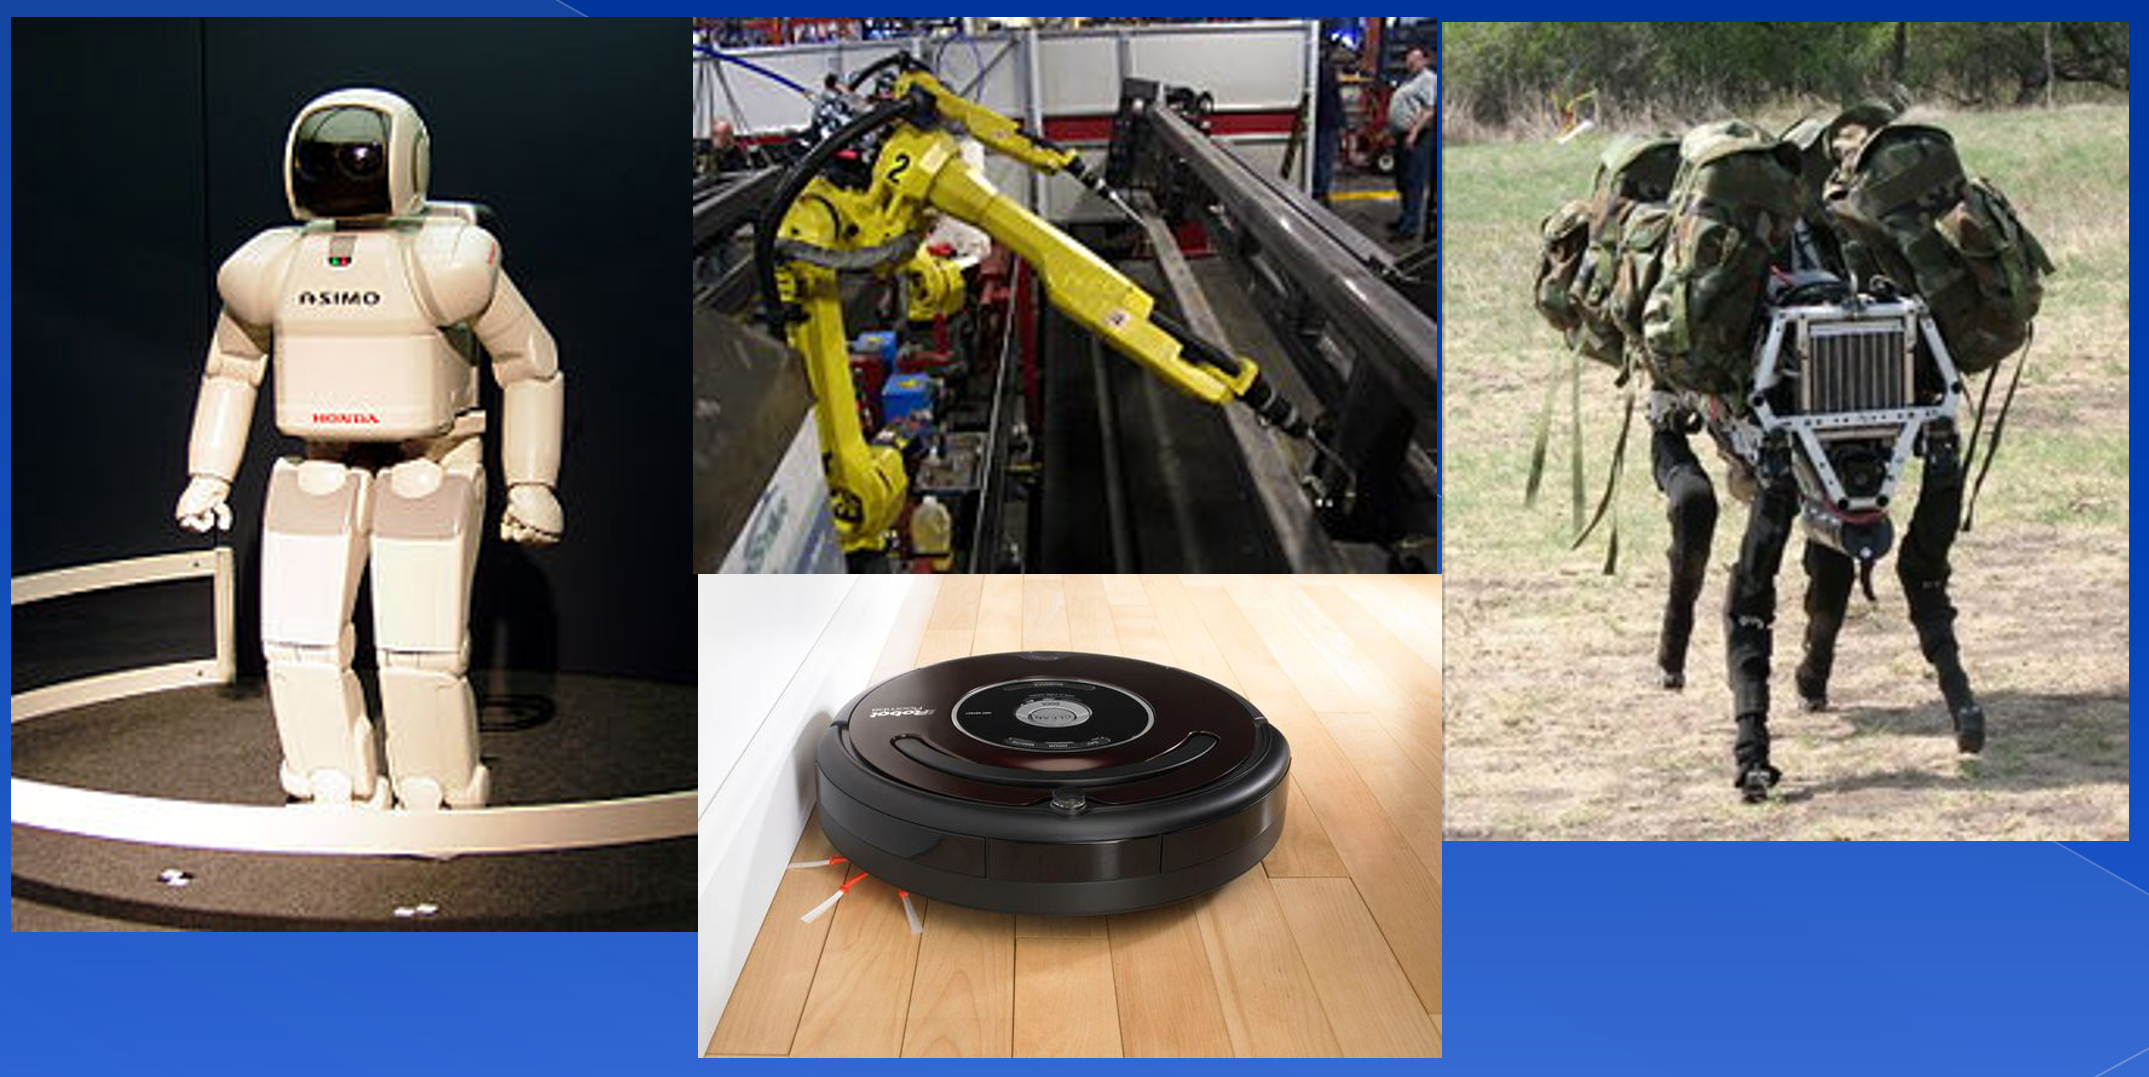
\includegraphics[width=0.75\linewidth]{robots.png}
\end{frame}

\begin{frame}
\frametitle{ИИ и роботы}
\onslide<1->{
\begin{itemize}
	\item Много примеров, когда робот есть, а ИИ - нет.
	\item И обратно, ИИ есть, а робота - нет.
\end{itemize}
}
\onslide<2->{
	\par\bigskip
	\centering
	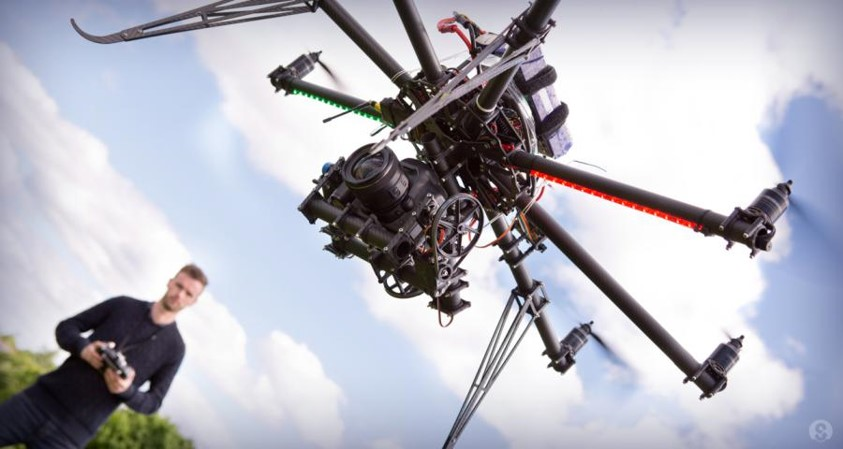
\includegraphics[height=0.27\linewidth]{dron.jpg}\hspace{10px} 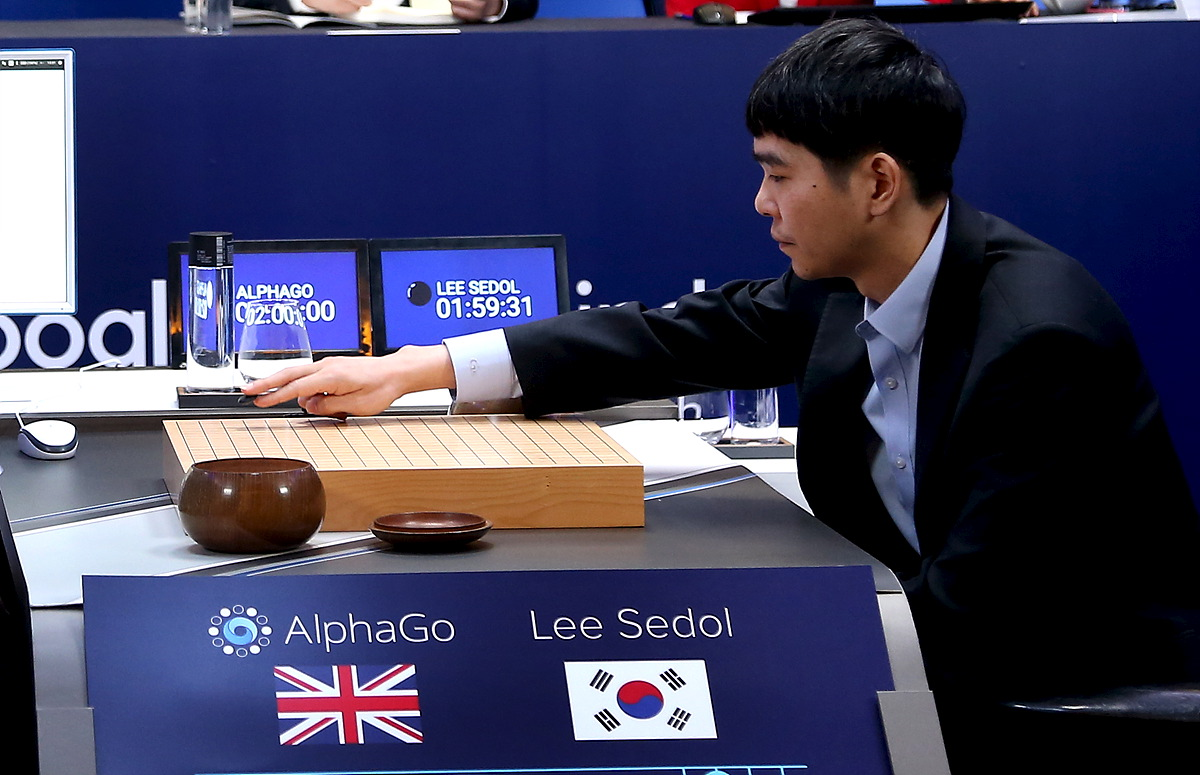
\includegraphics[height=0.27\textwidth]{alphago.jpg}
}
\end{frame}

\begin{frame}
	\frametitle{Что делает робота интеллектуальным?}
	Бихевиористский подход
	\begin{itemize}
		\item \textbf{Высокая степень автономности}
		
		\textit{Робот может самостоятельно (полностью или частично) функционировать в окружающей среде и решать поставленные задачи}
		
		\item \textbf{Возможность адаптации к изменяющейся среде}
		
		\textit{Каждый раз когда среда меняется робот самостоятельно меняет свое поведение}
		
		\item \textbf{Возможность взаимодействия с другими роботами}
		
		\item \textbf{Возможность взаимодействия с человеком}
	\end{itemize}
\end{frame}

\begin{frame}
	\frametitle{Методы ИИ и робототехника}
	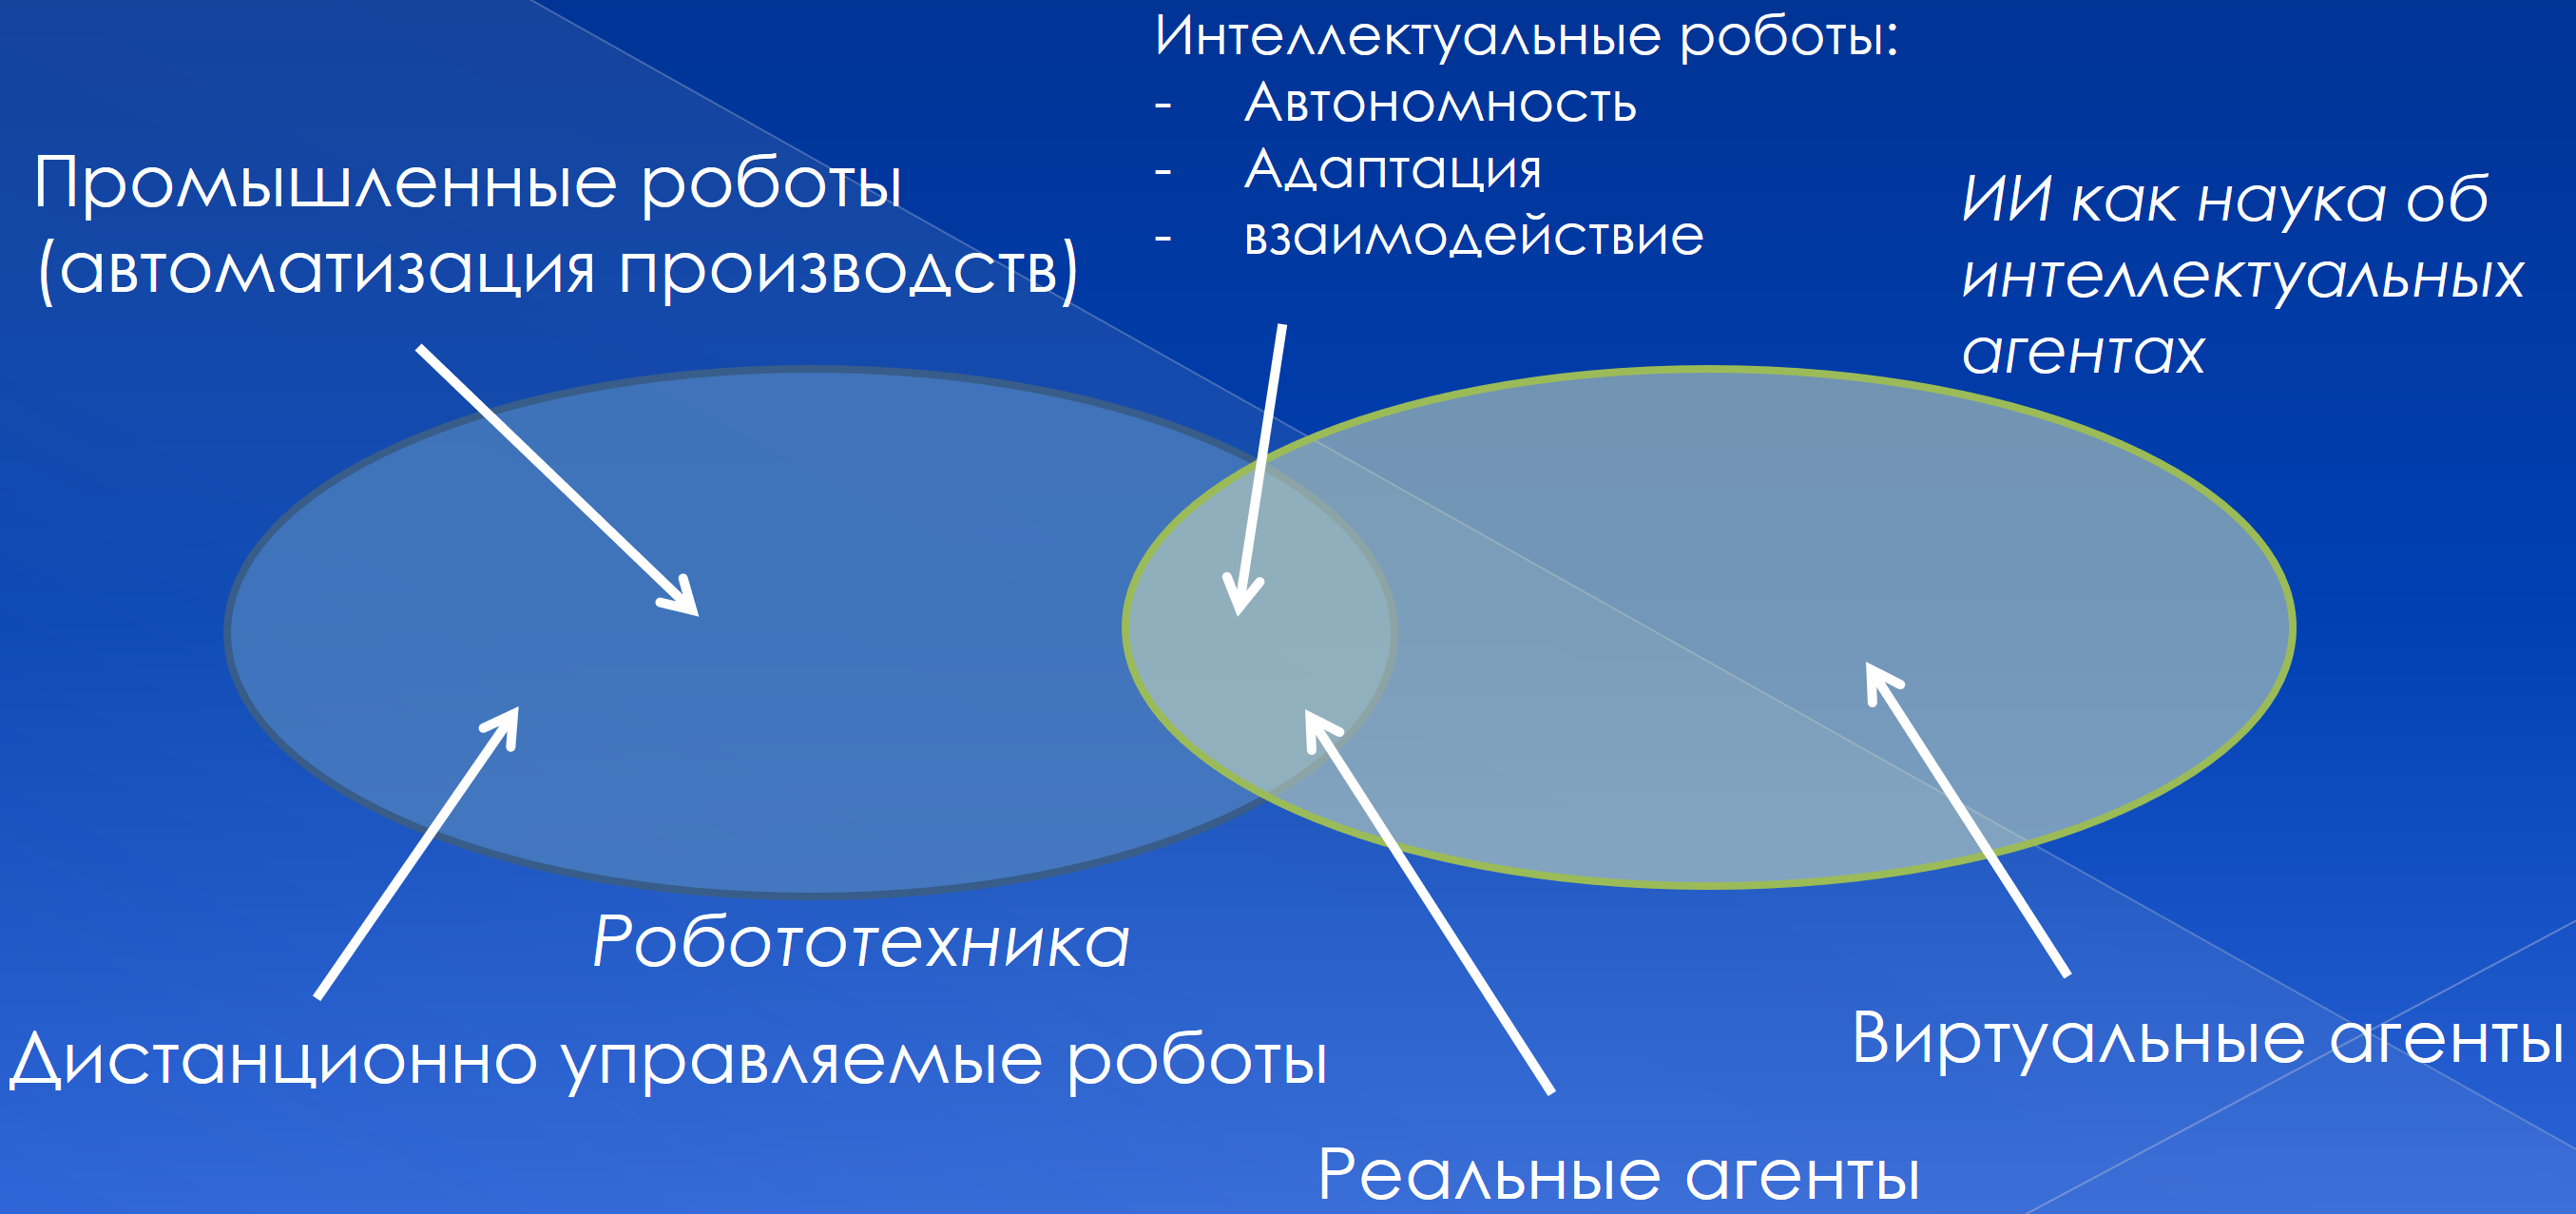
\includegraphics[width=\textwidth]{airobots.png}
\end{frame}

\begin{frame}
\frametitle{Интеллектуальные агенты и роботы}
\begin{itemize}
	\item Робот (железо) - тело агента:
	\begin{itemize}
		\item датчики (гироскоп, акселерометр, барометр, видео-камера, лидар, GPS приемник),
		\item актуаторы (манипулятор, колеса).
	\end{itemize}
	\item ИИ (программа) - мозг агента, который должен
	\begin{itemize}
		\item воспринимать окружающую действительность,
		\item обучаться, получать знания, представлять знания,
		\item рассуждать,
		\item планировать свое поведение,
		\item общаться с человеком и другими агентами,
		\item и т.д.
	\end{itemize}
\end{itemize}
\centering
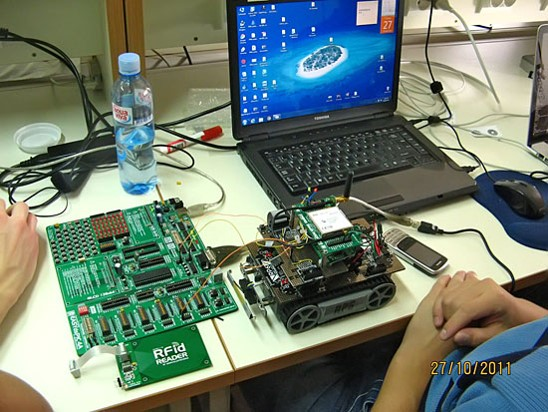
\includegraphics[width=0.3\textwidth]{schema.jpg}
\end{frame}

\section{Архитектуры управления и системный анализ}

\begin{frame}
\frametitle{План на сегодня}
\tableofcontents[currentsection] 
\end{frame}

\begin{frame}
\frametitle{Когнитивные архитектуры}
\begin{center}
	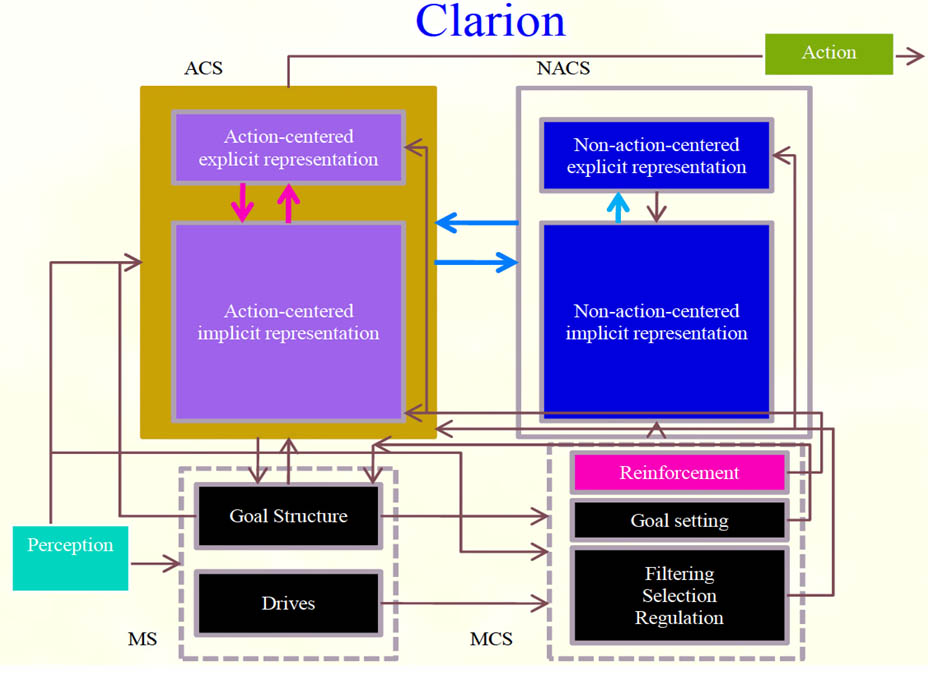
\includegraphics[width=0.4\textwidth]{agent-schemas/en/clarion.jpg}
	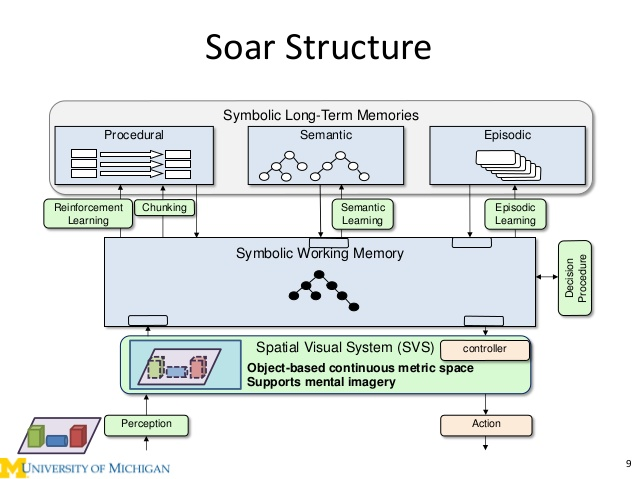
\includegraphics[width=0.4\textwidth]{agent-schemas/en/soar.jpg}
\end{center}
\scriptsize
Недостатки современных когнитивных архитектур:
\begin{itemize}
	\item Концептуальная нерешенность проблемы привязки символов (symbol grounding problem) - CLARION
	\item Отсутствие деятельностной модели поведения системы - реализация только некоторых когнитивных аспектов
	\item Иерархичность представления знаний (4D/RCS)
	\item Возможность реализации иерархического планирования
	\item Реализация обучения концептуальным знаниям - Cognitive Mario
	\item Моделирование рефлексивного поведения
\end{itemize}
\end{frame}

\begin{frame}
\frametitle{Архитектура STRL}
\begin{center}
	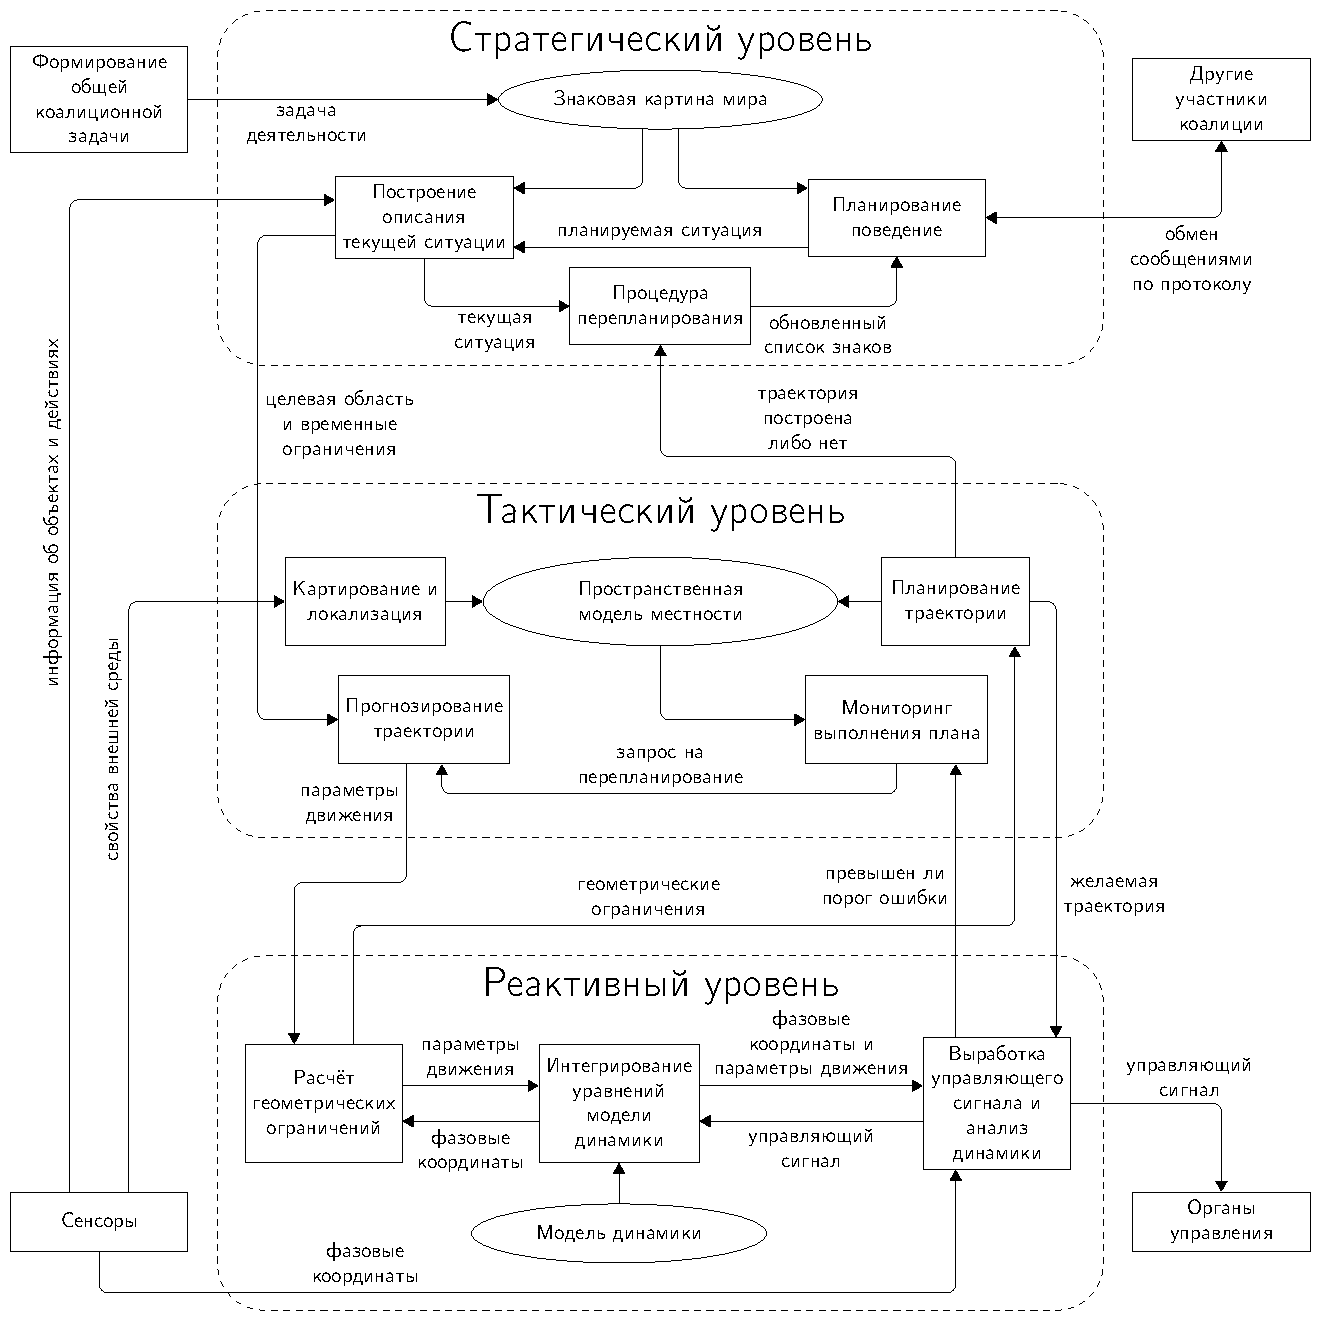
\includegraphics[width=0.7\textwidth]{agent-schemas/ru/architecture}
	
\end{center}
\end{frame}

\section{Решаемые задачи}
\begin{frame}
\frametitle{План на сегодня}
\tableofcontents[currentsection] 
\end{frame}

\begin{frame}
\frametitle{Задачи реактивного уровня}
\begin{itemize}
	\item Непосредственное взаимодействие со средой (моделирование в Gazebo).
	\item Построение и идентификация модели объекта управления.
	\item Решение задач стабилизации, следования и т.п., разработка регуляторов.
\end{itemize}
\par\bigskip
\begin{center}
	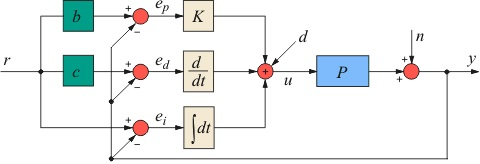
\includegraphics[width=0.7\textwidth]{pid.jpg}
	
\end{center}
\end{frame}

\begin{frame}
\frametitle{Задачи реактивного уровня}
\begin{itemize}
	\item Непосредственное взаимодействие со средой (моделирование в Gazebo).
	\item Построение и идентификация модели объекта управления.
	\item Решение задач стабилизации, следования и т.п., разработка регуляторов.
\end{itemize}
\par\bigskip
\begin{center}
	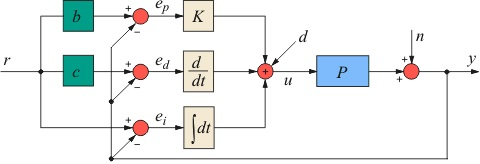
\includegraphics[width=0.6\textwidth]{pid.jpg}
	
\end{center}
\end{frame}

\begin{frame}
\frametitle{Задачи тактического уровня}
\begin{itemize}
	\item Картирование по видеопотоку.
	\item Локализация в построенной карте.
	\item Планирование траектории в динамической и\\или неизвестной среде.
	\item Планирование траекторий для множества агентов, избегание столкновений.
\end{itemize}
\par\bigskip
\begin{center}
	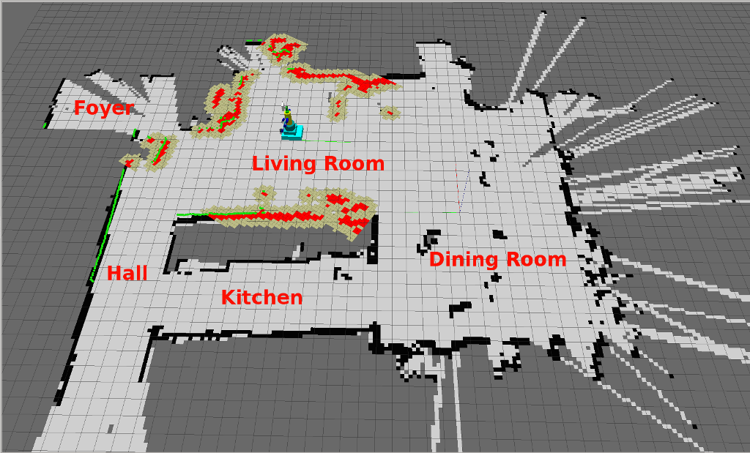
\includegraphics[width=0.6\textwidth]{loca.png}
	
\end{center}
\end{frame}


\begin{frame}
\frametitle{Задачи стратегического уровня}
\begin{itemize}
	\item Приобретение знаний (обучение, в т.ч. с подкреплением).
	\item Представление знаний как объективных, так и субъективных.
	\item Планирование поведения, в т.ч. в коалиции агентов.
	\item Моделирование мета-когнитивных функций (рефлексия, целеполагание и др.).
	\item Логический вывод и моделирование рассуждений.
\end{itemize}
\par\bigskip
\begin{center}
	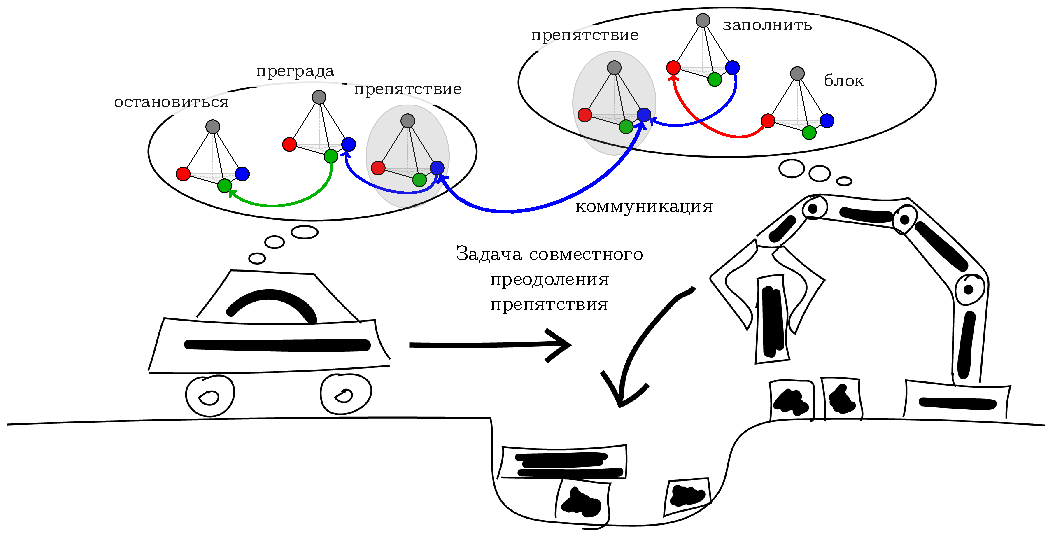
\includegraphics[width=0.6\textwidth]{robotic_signs}
	
\end{center}
\end{frame}

\begin{frame}
\frametitle{Темы проектов, курсовых и дипломных работ}
\tiny
\begin{itemize}
	\item Принцип гарантированного управления и его применение в нелинейных задачах.
	\item Приближенное решение задачи нелинейного управления на конечном интервале регулирования и его применение.
	\item Фильтрация в нелинейных системах.
	\item Сравнение эффективности различных нелинейных законов управления.
	
	\item Методы и алгоритмы эвристического поиска.
	\item Планирование траектории в виртуальных мирах как задача эвристического поиска пути на графе особой структуры.
	\item Планирование траектории беспилотных транспортных средств: методы и алгоритмы.
	\item Планирование траектории перемещения в пространстве положений для сложных робототехнических систем (манипуляторов и др.).
	\item Задачи картирования и локализации для беспилотных транспортных средств.
	\item Картирование и локализация для беспилотных летательных аппаратов по данным инерциальной навигационной системы и видеопотоку.
	\item Методы и алгоритмы выделения особенностей на растровых изображениях (SURF, SIFT  и др.).
	\item Методы и алгоритмы обработки изображений для робототехники.
	
	\item Обучение с подкреплением по модели Actor-Critic.
	\item Иерархическое обучение с подкреплением.
	\item Глубокое обучение с подкреплением.
	\item Обучение с подкреплением для манипулятора по видеопотоку.
	\item Нейросимвольные способы представления и приобретения знаний.
	\item Планирование поведения в коалиции агентов с распределением ролей.
	\item Нейробайесовские методы обучения.
	
\end{itemize}
\end{frame}

\begin{frame}

\centering
Спасибо за внимание!

\end{frame}

\end{document} 